\begin{frame}{Experiment 3}
\setbeamercovered{invisible}
\fontsize{11pt}{15}\selectfont


\only<1>{
\begin{figure}
    \centering
    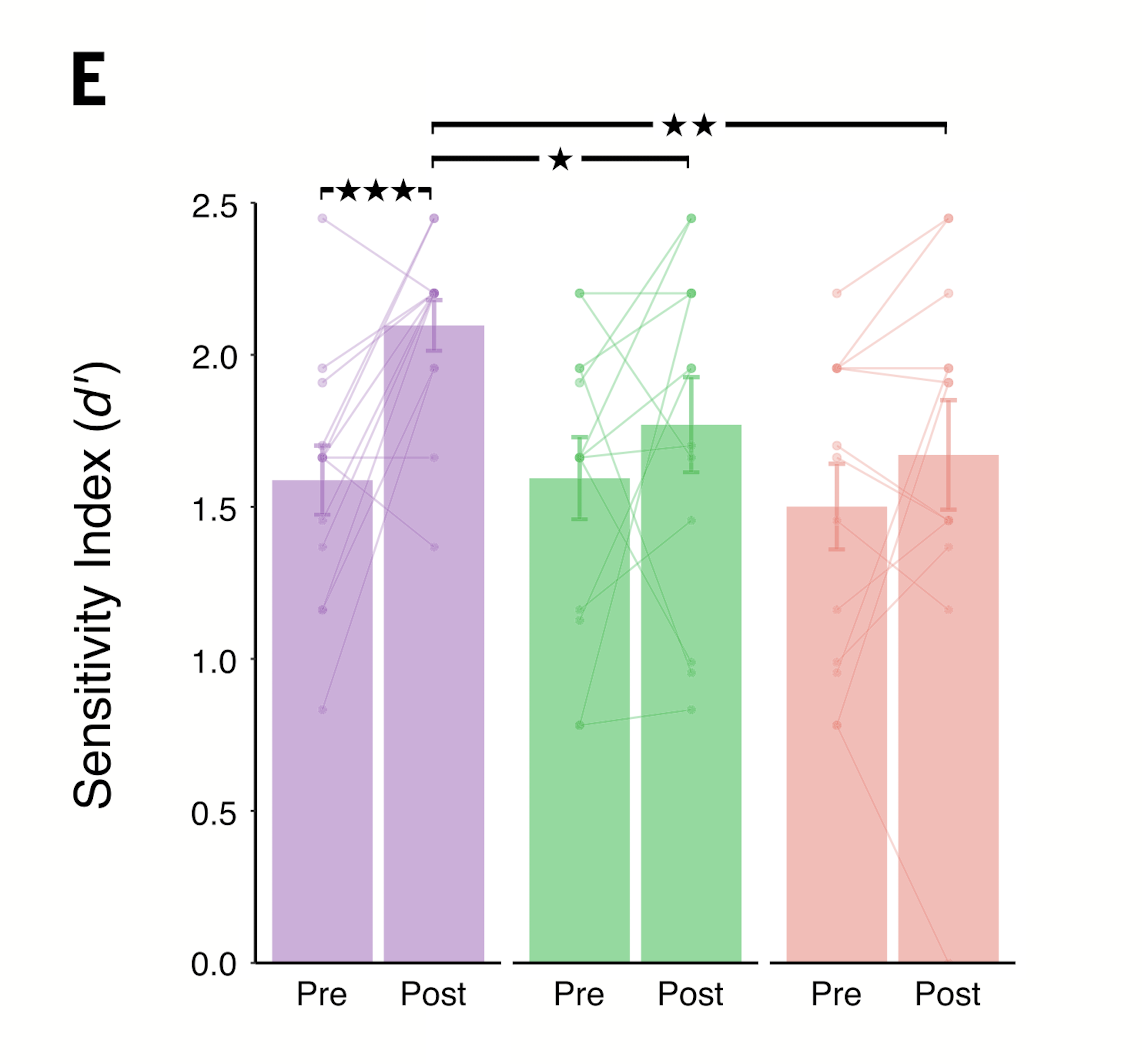
\includegraphics[width=6.5cm]{images/paper_pics/fig3E.png}
    \caption*{Participants improved for \textbf{object relatives} in the syntactic task (purple), but not after training with the free hand (green) or with the constrained hand (red)}
    \label{fig:label9}
\end{figure}
}

\pause
\only<2>{
{\large\textbf{Results:}}
\begin{itemize}
    \item Reconfirmed that \textbf{tool-use training} selectively \textbf{improved} comprehension of object relatives
    \item \textbf{Neither} free-hand training nor constrained-hand training significantly \textbf{enhanced} the performance for object relatives
    \item \textbf{After training}, the tool-use group significantly \textbf{outperformed} the others on object relatives comprehension
\end{itemize}
}

\end{frame}
